\subsection{Positive Ordered Integers Array:}

The first test will consist in evaluate the running time of the algorithms analyzing an array of ordered integers of size $2^{10}$. \hfill \break

{\bfseries\itshape\color{carmine}{Observation:}} {\itshape\color{carmine}{Since the size it's $2^{10}$ the parameters of the points of each algorithm are to many, so we decide to not attach only for this case the table of mapping values and the console output.}} \hfill \break

\begin{figure}[H]
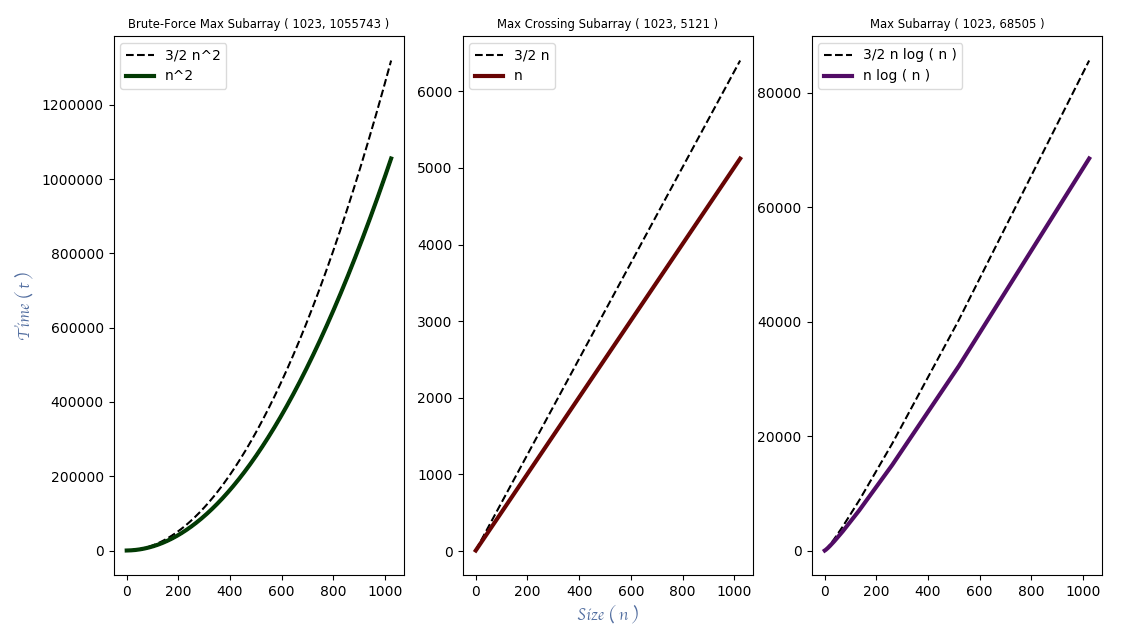
\includegraphics[width = 16.5cm, height = 8cm]{t1.png}
\centering \linebreak \linebreak Figure 4.1.0: Algorithms results for an array of size $2^{10}$.
\end{figure}

The second test will consist in evaluate the running time of the algorithms analyzing an array of ordered integers of size $2^{6}$. \hfill \break
